\documentclass[11pt, oneside]{article}   	% use "amsart" instead of "article" for AMSLaTeX format
\usepackage{geometry}                		% See geometry.pdf to learn the layout options. There are lots.
\geometry{letterpaper}                   		% ... or a4paper or a5paper or ... 
%\geometry{landscape}                		% Activate for for rotated page geometry
%\usepackage[parfill]{parskip}    		% Activate to begin paragraphs with an empty line rather than an indent
\usepackage{graphicx}				% Use pdf, png, jpg, or eps� with pdflatex; use eps in DVI mode
								% TeX will automatically convert eps --> pdf in pdflatex		
\usepackage{amssymb}
\usepackage{amsmath}
\usepackage{hyperref}

\title{Archimedes and pi}
%\author{The Author}
\date{}							% Activate to display a given date or no date

\graphicspath{{/Users/telliott_admin/Dropbox/Tex/png/}}

\usepackage{listings,relsize} 
\lstloadlanguages{R} 
\lstset{language=R,basicstyle=\smaller[1],commentstyle=\rmfamily\smaller, 
  showstringspaces=false,% 
  xleftmargin=4ex,literate={<-}{{$\leftarrow$}}1 {~}{{$\sim$}}1} 
\lstset{escapeinside={(*}{*)}}   % for (*\ref{ }*) inside lstlistings (S code) 

\begin{document}

\maketitle
%\section{}
% \subsection*{R code}
% \begin{lstlisting}  \end{lstlisting}
% \begin{center} 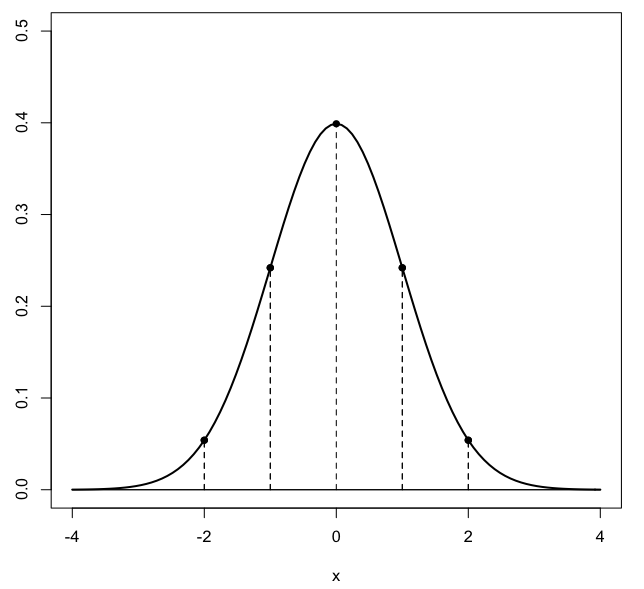
\includegraphics [scale=0.4] {gauss3.png} \end{center}
% \begin{bmatrix} a  &  b \\ c  &  d \end{bmatrix}
% \bigg |_

\large
This short write-up is an explanation of Archimedes' method for finding an approximation to the irrational number $\pi$.  The method uses \emph{inscribed} and \emph{circumscribed} polygons around a circle.  The circle has a diameter equal to $1$ and so its circumference is equal to $\pi$.

We will approximate the the value of $\pi$ by squeezing it between two other values, the perimeter of the inscribed polygon, which is less than the circumference, and the perimeter of the circumscribed polygon, which is greater than the circumference.

The figure below shows a sketch of the polygons when $n=8$.  We will be increasing the number of sides by a factor of $2$ at each step, so these are really $2^n$-gons.  Here, $n=3$.
\begin{center} 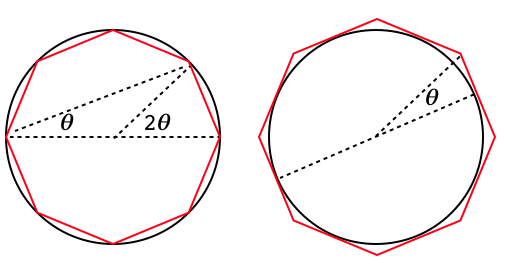
\includegraphics [scale=0.6] {pi.png} \end{center}

\subsection*{Finding perimeters in terms of angle $\theta$}

For the left panel, we have $8$ sides, so the central angle (marked $2\theta$) is equal to $45^\circ$, and $\theta$ is one-half that.  By a standard theorem, the larger triangle with angle $\theta$ is a right triangle, so the length of the inscribed n-gon side is $S = sin \ \theta$, since the hypotenuse of the triangle is the diameter of the circle, which is equal to $1$.  The total perimeter is $2^n=8$ times S.

For the right panel, we have just rotated the diameter a little bit, it's the same circle, but with n-gons outside, circumscribing the circle.  So the angle marked $\theta$ is half the angle we marked as $2 \theta$ previously since the diameter comes down to the middle of the side.  It has the same measure as $\theta$ from before, and the length of the half-side for that triangle is $(1/2)T$ divided by $1/2$ (the half diameter) and so equals $ tan \ \theta$.  But that means $T = tan \ \theta$.

So all of this gives us two equations, at each stage there are $2^n$ sides, the length of each short side $S$ on the inside equals $sin \ \theta$ and the length of each short side on the outside $T$ is equal to $tan \ \theta$.  $S$ and $T$ are equal to the sine and tangent of the angle $\theta$, where $\theta = 180/2^n$.
\subsection*{The base case}

If we go back to the square ($n=2, 2^n = 4$), then the total perimeter of the outside n-gon is equal to $4$ times the diameter $= 4 = 4T$ (so $T=1$), while the total perimeter of the inside n-gon is equal to $4/ \sqrt{2} = 4S$ (so $S = 1/\sqrt{2}$), which is correct.  $\angle \ \theta = 45^\circ$ and its tangent is $1$ and its sine is $1/\sqrt{2}$.

Now, what we are going to do is to increase $n$ in steps of 1, that increases $2^n$ by a factor of $2^1 = 2$ each time, which halves the angle.  All we need is a way to compute trigonometric functions of $\theta/2$, knowing the values for $\theta$, so we can calculate what happens to the perimeter.

\subsection*{Half angle formulas}

Recall the sum of angles formula (we derived these elsewhere).  Let's do cosine first
\[ cos(x+y) = cos \ x \ cos \ y -  sin \ x \ sin \ y \]
if $x=y$ then
\[ cos \ 2x = cos^2x - sin^2x = 2 \ cos^2x - 1 \]
\[ cos^2x = \frac{1}{2}(1 + cos\ 2x) \]
\[ cos \ x = \sqrt{\frac{1 + cos\ 2x}{2}}\]
And
\[ sin(x+y) = sin \ x \ cos \ y +  sin \ y \ cos \ x \]
if $x=y$ then
\[ sin \ 2x = 2 \ sin \ x \ cos \ x \]
\[ sin \ x = \frac{1}{2} \ sin \ 2x  \ \frac{1}{cos \ x} =  \frac{1}{2} \ sin\ 2x \ \sqrt{\frac{2}{1+cos\ 2x}}\]

So if we know $cos\ 2x$ we can use the first formula to get $cos \ x$ and then apply the second to get $sin \ x$.  Finally, divide to get the tangent.

\subsection*{Simpler formulas}

Suppose we know all the values---sine, cosine and tangent---given angle $\theta$---for some value of $n$.  Let us designate them as $S$, $C$ and $T$, and we will then substitute $\theta = 2x$.  Using the above formulas, we can calculate $cos \ x$, etc.  Let's designate these values for the half-angle as C', S' and T'.
On the web pages that got me started with this derivation
\vspace{2 mm}

\noindent \url{http://personal.bgsu.edu/~carother/pi/Pi3d.html}
\vspace{2 mm}

\noindent there is a simpler pair of formulas listed, namely, for an inside perimeter of $p$ and an outside perimeter of $P$
\[ P' = \frac{2pP}{p + P} \]
\[ p' = \sqrt{pP'} \]
�which means that $P'$ is the \emph{harmonic mean} of $p$ and $P$, while $p'$ is the geometric mean of $p$ and $P'$.  I thought it would be worthwhile to demonstrate the connection.  

I have to admit I puzzled over it for a while, the reason is that I confused these formulas for the perimeters, with the formulas we develop below, which are for the sine and tangent of the angle.
\subsection*{Onward}
We have
\[ sin \ x = \frac{1}{2} \ sin \ 2x  \ \frac{1}{cos \ x} \]
\[ S' = \frac{1}{2} \ S \ \frac{1}{C'} \]
also
\[ cos^2x = \frac{1}{2}(1 + cos\ 2x) \]
\[ (C')^2 = \frac{1}{2}(1+C) = \frac{1+C}{2} \]
The first formula from the website is for $T'$
\[ T' = \frac{S'}{C'} = \frac{1}{2} \ S \ \frac{1}{C'} \ \frac{1}{C'} = \frac{1}{2} \ S \ \frac{2}{1+C} =  \frac{S}{1+C}\]
multiply top and bottom by $T$
\begin{equation}
\boxed{ T' =  \frac{ST}{S+T}}
\end{equation}
For the second one
\[ S' = \frac{1}{2} \ S \ \frac{1}{C'} =  \frac{1}{2} \ S \ \frac{T'}{S'} \]
\begin{equation}
\boxed{ S' = \sqrt{\frac{ST'}{2}}}
\end{equation}
Let's try checking the results for a known angle
\[ 2x = \pi/3, \ sin = \frac{\sqrt{3}}{2}, \ cos = \frac{1}{2}, \ tan = \sqrt{3} \]
\[ x = \pi/6, \ sin = \frac{1}{2}, \ cos = \frac{\sqrt{3}}{2}, \ tan = \frac{1}{\sqrt{3}} \]
Our first equation is
\[ T' =  \frac{ST}{S+T} = \frac{3/2}{(3/2)\sqrt{3}} = \frac{1}{\sqrt{3}} \]
That looks good.  The second one is
\[ S' = \sqrt{\frac{ST'}{2}} \]
\[ ST' = \frac{\sqrt{3}}{2} \frac{1}{\sqrt{3}} = \frac{1}{2} \]
\[ S' = \sqrt{ \frac{1}{2}\ \ \frac{1}{2}} = \frac{1}{2} \]
These both look correct.
\subsection*{Resolution}
Just a brief reminder about nomenclature.  We have $P$ and $p$, the perimeters of the circumscribed n-gon and the inscribed n-gon.  We have $S$ and $T$, for the sine and cosine of the angle (as described above).  And we use a prime $'$ to designate the $n+1$ version of each of these values, compared with the current version which is the $n$ version.  And at each stage we have that 
\[ p = 2^n S \]
\[ P = 2^n T \]

We also have our equations 
\[ T' =  \frac{ST}{S+T} \]
\[ S' = \sqrt{\frac{ST'}{2}} \]
and their equations
\[ P' = \frac{2pP}{p + P} \]
\[ p' = \sqrt{pP'} \]
and we need to reconcile them.

Start with
\[ P' =  2^{n+1} \ T'= 2^{n+1} \ \frac{ST}{S+T} \]
\[ = 2 \ 2^{n} \ \frac{2^n}{2^n} \ \frac{ST}{S+T} \]
\[ = 2 \frac{2^nS \ 2^n T}{2^n (S + T)}\]
\[ = 2 \frac{pP}{p + P}\]
So, we gain a factor of two, as we needed.  And
\[ (S')^2 = \frac{ST'}{2} \]
\[ (p')^2 = 2^{n+1} \ 2^{n+1} \ (S')^2 = 2 \ 2^n \ 2^{n+1} \frac{ST'}{2} \]
\[ = 2 \frac{2^n S \ 2^{n+1}T'}{2} =  2 p P / 2 = p P' \]
\[ p' = \sqrt{p P'} \]
As stated.

Now, I think we should run a simulation to see what kind of numbers we get.  We start with the square ($n=2$, $2^n = 4$)
Previously we found that $S=1/\sqrt{2}$ and $T=1$ so
\[ p = 2^n S = \frac{4}{\sqrt{2}} = 2.8284 \]
\[ P = 2^n T = 4 \]
Let's try a script to calculate this to larger $n$.
\Large
\begin{lstlisting}
p = 4.0/(2**0.5)
P = 4

def one_round(t):
    p,P = t
    P2 = 2*p*P/(p+P)
    p2 = (p*P2)**0.5
    return p2,P2

s = '%3.10f  %3.10f'
print '%2d' % 1, s % (p,P)
for i in range(18):
    p,P = one_round((p,P))
    if not i%3:
        print '%2d' % (i+2), s % (p,P)
        
Output:
> python pi.py
 1 2.8284271247  4.0000000000
 2 3.0614674589  3.3137084990
 5 3.1403311570  3.1441183852
 8 3.1415729404  3.1416320807
11 3.1415923456  3.1415932696
14 3.1415926488  3.1415926632
17 3.1415926535  3.1415926537

\end{lstlisting}
\large
That looks pretty good to me.

\end{document}  